\section*{Problem 1}

\begin{enumerate}
    \item
    First note that the system is in controllable canonical form. Thus, the transfer function from $u(k)$ to $Cx(k)$ is
    \begin{align*}
        G(z) = \frac{ z - 1.25 }{ z^2 - 0.3 z - 0.4 } 
            = \frac{ z - 1.25 }{ (z - 0.8)(z + 0.5) }
    \end{align*}
    The reciprocal root locus plot for this LQR design is shown in Figure~\ref{fig:finalp1_rl1}.
    \begin{figure}
        \centering
        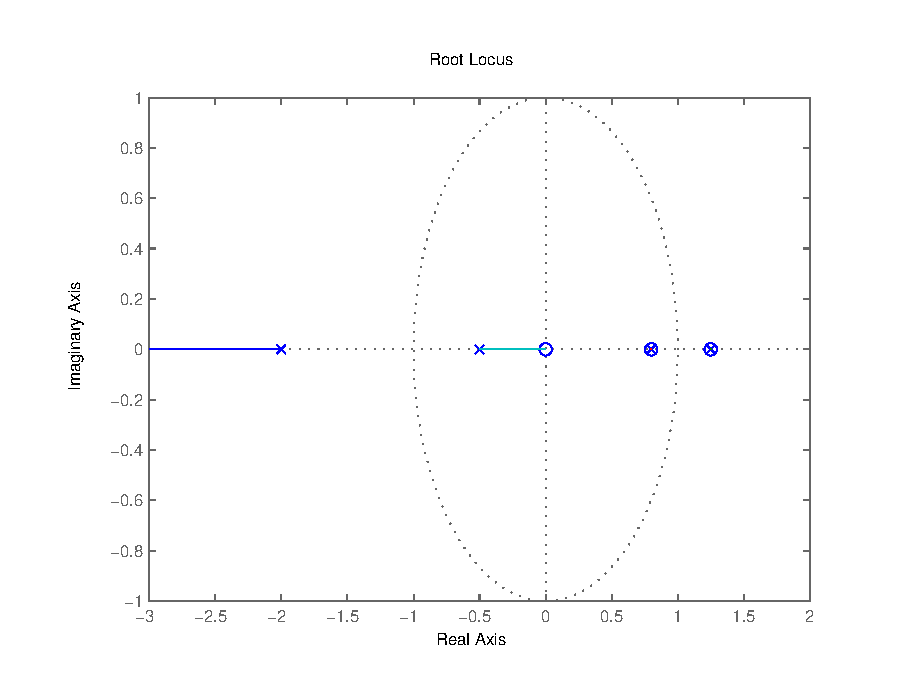
\includegraphics[width=8cm]{finalp1_rl1}\\
        \caption{Reciprocal root locus plot for Problem 1, part 1}
        \label{fig:finalp1_rl1}
    \end{figure}
    Note that, regardless of how $R$ is chosen, the closed-loop system always has a pole at $z = 0.8$.
    
    \item
    Since the closed-loop poles converge to the open-loop zeros of $G$ (or their inverses) as $R \rightarrow 0$, it is sufficient to choose the zeros so that they both have magnitude less than $0.5$. Regardless of how $C$ is chosen, $G(z)$ will always have relative degree of at least 1, so there will always be a zero at the origin. By choice of $C$, we can choose the location of the other zero. For instance, putting a zero at $z=0.4$, which corresponds to
    \begin{align*}
        C = \begin{bmatrix}
                -0.4 & 1
            \end{bmatrix}
    \end{align*}
    results in the reciprocal root locus plot shown in Figure~\ref{fig:finalp1_rl2}.
    \begin{figure}
        \centering
        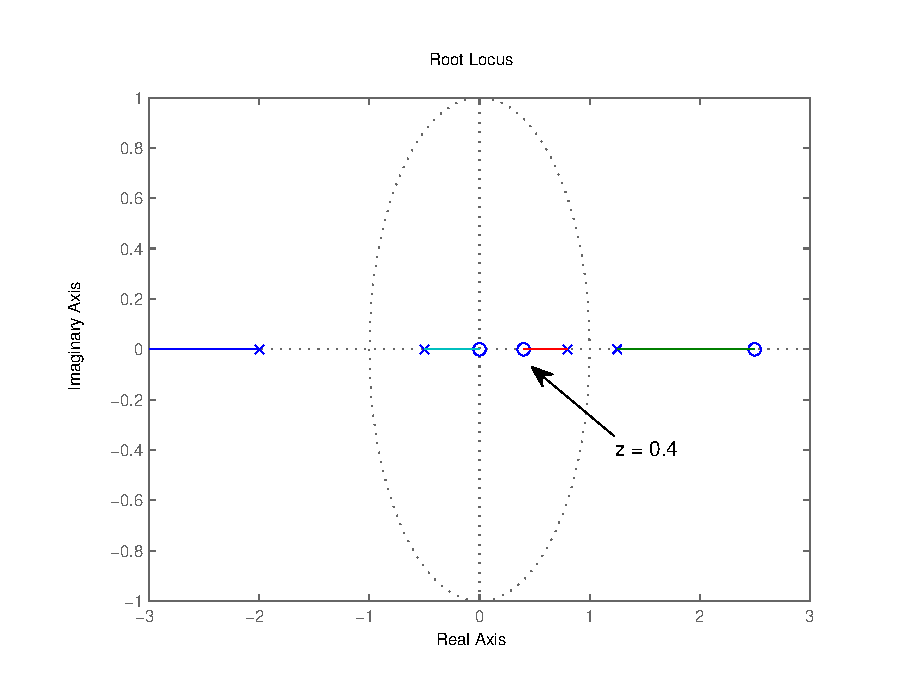
\includegraphics[width=8cm]{finalp1_rl2}\\
        \caption{Reciprocal root locus plot for Problem 1, part 2}
        \label{fig:finalp1_rl2}
    \end{figure}    
    Note that as $R \rightarrow 0$, the closed-loop poles converge to $0$ and $0.4$.
    
\end{enumerate} 